\documentclass[handout]{beamer}
\usepackage[utf8]{inputenc}
\usepackage{graphicx}
\usepackage{booktabs}
\usepackage{array}
\usepackage{amsmath}

\usetheme{Cuerna}
\usecolortheme{default}

\setbeamertemplate{footline}{%
  \hfill\insertframenumber/\inserttotalframenumber\hspace{2mm}\vspace{2mm}%
}
\graphicspath{{../images/}{./}}

\logo{
\includegraphics[width=1.5cm]{bluesimplex.png}}
\title{Trajectory Classification with LSTM\\for Robotic Peg-in-Hole}
\author{Group 1 - LOUNAS Gana | MAGOUO NOCHI}
\date{Master's Machine Learning Project -- 2025--2026}
\institute{UE5 Apprentissage}

\begin{document}

\begin{frame}
  \titlepage
\end{frame}

\section{Introduction}
\begin{frame}{Project Objectives}
\small
\begin{itemize}[<+->]
  \item Build a trajectory-level classifier for a 7-DoF peg-in-hole task with \textbf{3 classes}.
  \item Use a sequence model aligned with course material (\textbf{RNN/LSTM} module).
  \item Deliver two outcomes required by the assignment:
  \begin{itemize}[<+->]
    \item strong performance on the internal test split,
    \item explicit analysis of \textbf{feature influence} on performance.
  \end{itemize}
\end{itemize}
\end{frame}

\begin{frame}{Problem Framing}
\small
\begin{itemize}[<+->]
  \item Input: one full trajectory tensor \(\in \mathbb{R}^{150 \times 20}\).
  \item Output: one class label \(\in \{0,1,2\}\) for the complete sequence.
  \item Why sequence learning: class information is encoded in \textbf{temporal dynamics}, not only static snapshots.
  \item Evaluation context: internal split (train/val/test) in notebooks, plus compatibility with teacher-held hidden test format.
\end{itemize}
\end{frame}

\begin{frame}{Roadmap}
\small
\begin{enumerate}[<+->]
  \item Data extraction and preparation
  \item Model
  \item Experimental plan (hyperparameters)
  \item Challenges encountered
  \item Results and analysis
  \item Feature consequences study
  \item Conclusion
\end{enumerate}
\end{frame}

\section{Data Extraction and Preparation}
\begin{frame}{Dataset and Feature Blocks}
\small
\begin{itemize}[<+->]
  \item Files: \texttt{class1\_trajectories.npy}, \texttt{class2\_trajectories.npy}, \texttt{class3\_trajectories.npy}
  \item Balanced data: \(256\) trajectories/class, total \(768\) trajectories.
  \item Shape per sample: \(150\) timesteps, \(20\) features.
  \item Labels: class1 \(\rightarrow 0\), class2 \(\rightarrow 1\), class3 \(\rightarrow 2\).
\end{itemize}
\vspace{0.3em}
\small
\begin{tabular}{lcc}
\toprule
\textbf{Block} & \textbf{Meaning} & \textbf{Size} \\
\midrule
\texttt{peg\_pose} & peg position + quaternion & 7 \\
\texttt{peg\_vel} & linear + angular velocity & 6 \\
\texttt{hole\_pos} & hole position + quaternion & 7 \\
\midrule
\textbf{Total} &  & \textbf{20} \\
\bottomrule
\end{tabular}
\end{frame}

\begin{frame}{Preprocessing Pipeline}
\small
\begin{itemize}[<+->]
  \item Reproducibility: fixed random seed (\texttt{SEED=42}) for split and initialization.
  \item Split: \textbf{80/10/10} \(\Rightarrow\) train \(614\), val \(76\), test \(78\).
  \item Normalization: z-score computed on train only, then reused on val/test.
  \item Numerical stability: \(\sigma = 0\) replaced by small \(\epsilon\).
\end{itemize}
\vspace{-0.1em}
\[
\mathbf{x}_{norm} = \frac{\mathbf{x}-\boldsymbol{\mu}_{train}}{\boldsymbol{\sigma}_{train}+\epsilon}
\]
\vspace{-0.2em}
\small
\begin{itemize}[<+->]
  \item This prevents leakage and improves optimization conditioning.
\end{itemize}
\end{frame}

\begin{frame}{Trajectory Evidence Before Training}
\begin{columns}[t,onlytextwidth]
  \column{0.48\textwidth}
  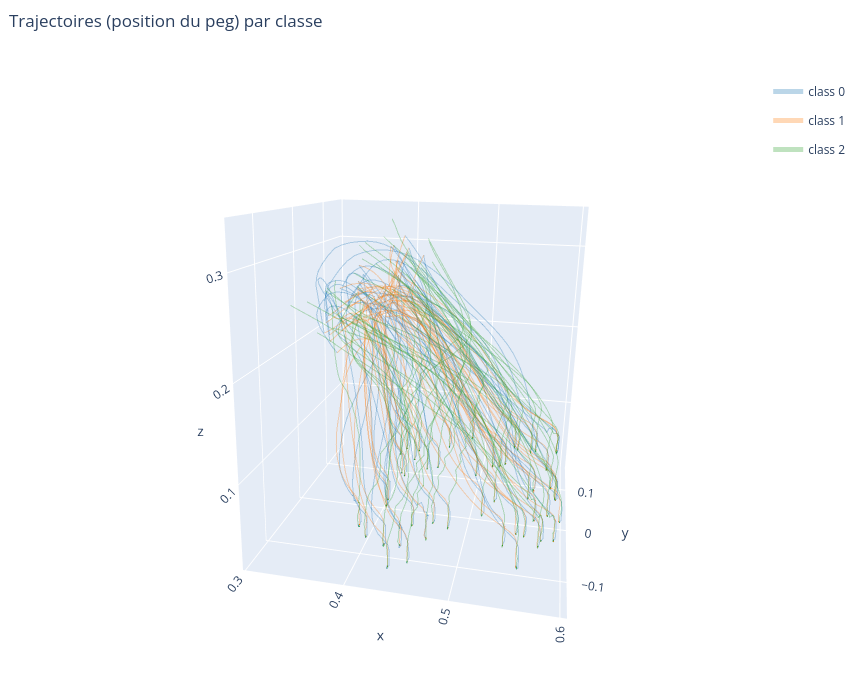
\includegraphics[width=\linewidth]{3D_viz_data.png}
  {\scriptsize 3D trajectories (\(x,y,z\)) by class.}
  \column{0.48\textwidth}
  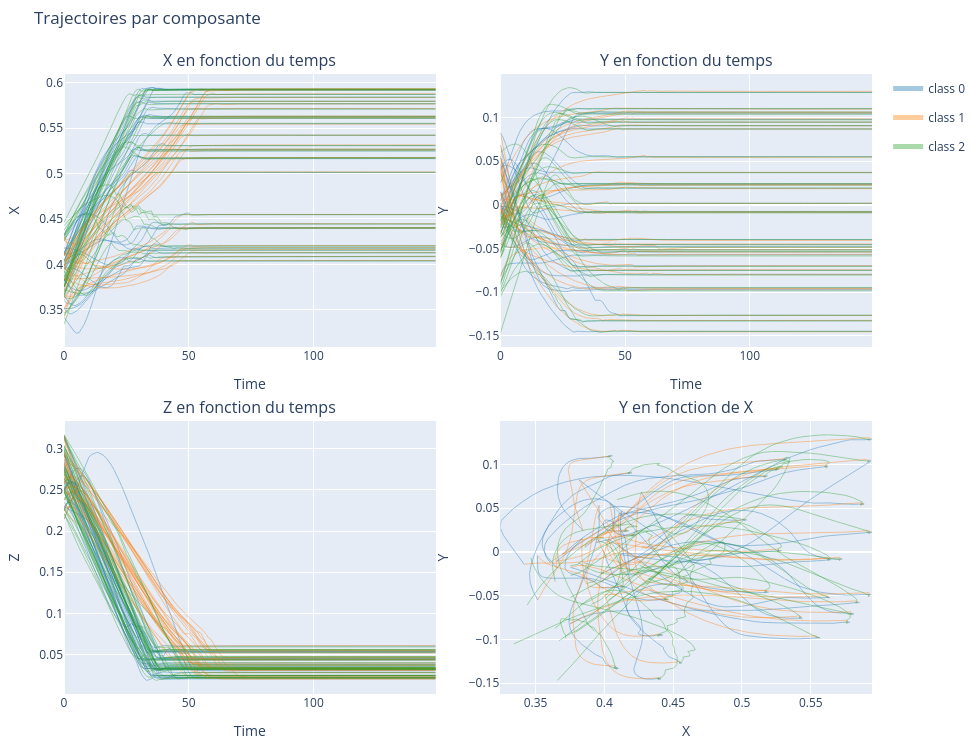
\includegraphics[width=\linewidth]{2D_viz_data.png}
  {\scriptsize Projections: \(x(t), y(t), z(t), y(x)\).}
\end{columns}
\vspace{0.3em}
\small
Class-dependent temporal patterns are visible before training, which motivates a temporal classifier.
\end{frame}

\section{Model}
\begin{frame}{Why LSTM (Course Connection)}
\small
\begin{itemize}[<+->]
  \item Course reminder (\texttt{3\_RNN\_Transformers\_2025.pdf}): vanilla RNNs are sensitive to vanishing/exploding gradients through BPTT.
  \item LSTM uses gated memory to control information flow and preserve useful long-range signals.
\end{itemize}
\vspace{-0.2em}
\[
i_t,f_t,o_t=\sigma(\cdot),\quad \tilde{c}_t=\tanh(\cdot),\quad
c_t=f_t\odot c_{t-1}+i_t\odot \tilde{c}_t
\]
\vspace{-0.6em}
\small
\begin{itemize}[<+->]
  \item This architecture matches the project setting: long trajectories (\(150\) steps) with dynamic class signatures.
\end{itemize}
\end{frame}

\begin{frame}{Final Architecture and Training Setup}
\small
\begin{itemize}[<+->]
  \item Input tensor: \((\texttt{batch},150,20)\).
  \item Backbone: \texttt{LSTM(num\_layers=2, hidden\_size=64, dropout=0.2)}.
  \item Classifier head: last hidden state \(\rightarrow\) \texttt{Linear(64,3)}.
  \item Loss/optimizer: \texttt{CrossEntropyLoss} + \texttt{Adam(lr=1e-3)}.
  \item Batch size: \(32\), training budget up to \(40\) epochs in main experiments.
  \item Stability control: gradient clipping \(\|\nabla\|_{max}=1.0\).
\end{itemize}
\end{frame}

\section{Experimental Plan for Hyperparameters}
\begin{frame}{Controlled Experiment Plan}
\small
\begin{tabular}{>{\raggedright\arraybackslash}p{1.1cm} >{\raggedright\arraybackslash}p{4.1cm} >{\raggedright\arraybackslash}p{3.9cm}}
\toprule
\textbf{Run} & \textbf{Setting} & \textbf{Purpose} \\
\midrule
R1 & hidden=100, z-score, 10 epochs & baseline behavior \\
R2 & hidden=64, no normalization & sensitivity to scaling \\
R3 & hidden=64 + dropout & regularization impact \\
R4 & R3 + clipping & stability impact \\
\bottomrule
\end{tabular}
\vspace{0.4em}
\small
\begin{itemize}[<+->]
  \item Fixed controls: seed, split protocol, optimizer family, class definition.
  \item Selection criterion: best generalization with stable learning curves.
\end{itemize}
\end{frame}

\section{Challenges Encountered}
\begin{frame}{Practical Issues During Development}
\footnotesize
\begin{itemize}[<+->]
  \item \textbf{Reproducibility}: no fixed seed \(\Rightarrow\) difficult run-to-run comparison.
  \item \textbf{Optimization sensitivity}: preprocessing and regularization strongly alter convergence quality.
\end{itemize}
\begin{columns}[t,onlytextwidth]
  \column{0.48\textwidth}
  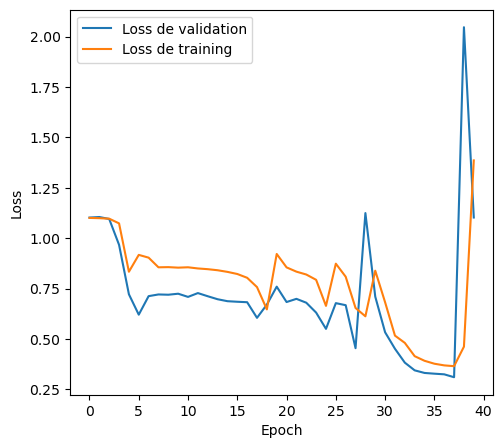
\includegraphics[width=0.95\linewidth]{sans_normalisation.png}
  {\scriptsize No normalization: noisier and less predictable convergence.}
  \column{0.48\textwidth}
  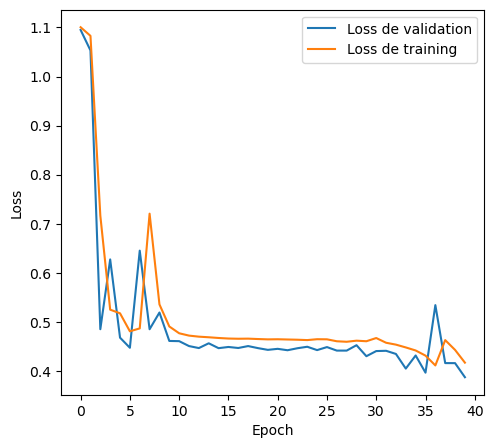
\includegraphics[width=0.95\linewidth]{no_dropout.png}
  {\scriptsize No dropout: weaker regularization and higher instability.}
\end{columns}
\end{frame}

\begin{frame}{Exploding Gradients and Mitigation}
\begin{columns}[t,onlytextwidth]
  \column{0.50\textwidth}
  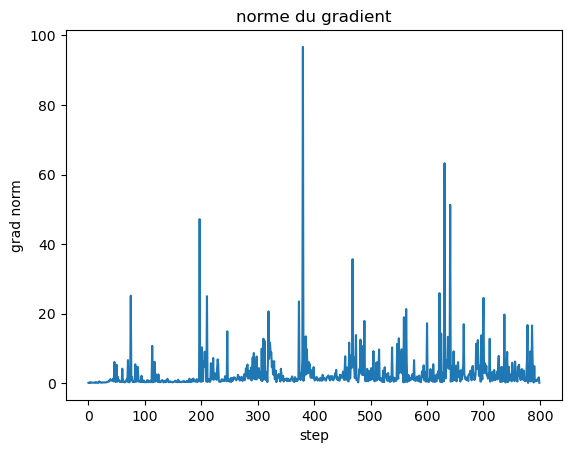
\includegraphics[width=0.90\linewidth]{gradient_explosion.png}
  {\scriptsize Gradient norm spikes observed during training.}
  \column{0.46\textwidth}
  \scriptsize
  \textbf{Observed issue}\\
  Large gradient spikes destabilize parameter updates.
  \vspace{0.2em}

  \textbf{Fix used}\\
  Gradient clipping in the training loop:\\
  \texttt{clip\_grad\_norm\_(..., 1.0)}.
  \vspace{0.2em}

  \textbf{Effect}\\
  More stable updates and smoother final convergence.
\end{columns}
\end{frame}

\section{Results and Analysis}
\begin{frame}{Main Runs R1 and R2}
\begin{columns}[t,onlytextwidth]
  \column{0.48\textwidth}
  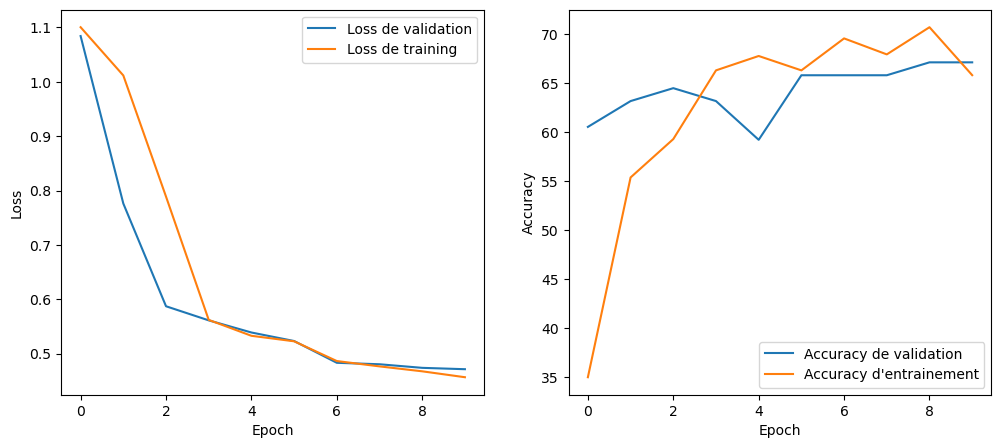
\includegraphics[width=\linewidth]{model_1_loss_accuracy.png}
  {\scriptsize R1 baseline: limited/unstable behavior.}
  \column{0.48\textwidth}
  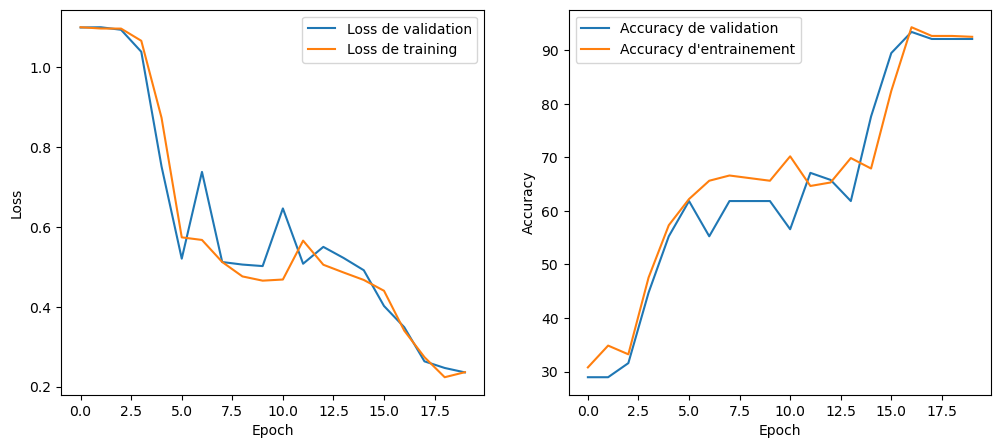
\includegraphics[width=\linewidth]{model_2_loss_accuracy.png}
  {\scriptsize R2: strong gain, \textbf{92.31\%} test accuracy (72/78).}
\end{columns}
\end{frame}

\begin{frame}{Main Runs R3 and R4}
\begin{columns}[t,onlytextwidth]
  \column{0.48\textwidth}
  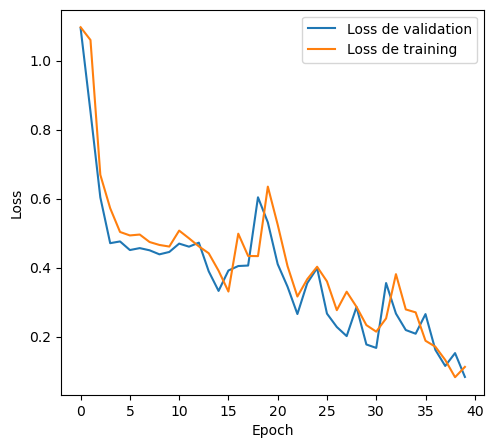
\includegraphics[width=\linewidth]{model_3_loss_accuracy.png}
  {\scriptsize R3 (+dropout): \textbf{98.72\%} test accuracy (77/78).}
  \column{0.48\textwidth}
  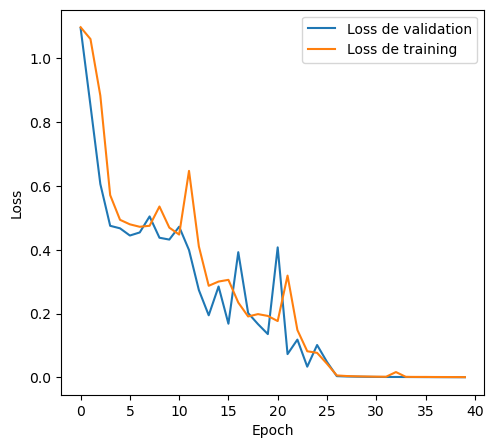
\includegraphics[width=\linewidth]{model_4_loss_accuracy.png}
  {\scriptsize R4 (+dropout + clipping): \textbf{100\%} (78/78).}
\end{columns}
\end{frame}

\begin{frame}{Quantitative Synthesis}
\small
\begin{tabular}{lcc}
\toprule
\textbf{Run} & \textbf{Test accuracy} & \textbf{Main effect} \\
\midrule
R1 & baseline (unstable) & underfitting/instability \\
R2 & 92.31\% (72/78) & better capacity choice \\
R3 & 98.72\% (77/78) & dropout improves generalization \\
R4 & 100.00\% (78/78) & clipping improves stability \\
\bottomrule
\end{tabular}
\vspace{0.5em}
\small
\begin{itemize}[<+->]
  \item Most impactful additions in this pipeline: \textbf{dropout + clipping}.
  \item Internal split performance is excellent; external hidden test remains the final robustness check.
\end{itemize}
\end{frame}

\section{Feature Consequences Study}
\begin{frame}{Feature-Ablation Protocol (Feature Notebook)}
\footnotesize
\setlength{\tabcolsep}{3pt}
\begin{tabular}{>{\raggedright\arraybackslash}p{2.2cm} >{\raggedright\arraybackslash}p{1.2cm} >{\raggedright\arraybackslash}p{1.8cm} >{\raggedright\arraybackslash}p{2.2cm}}
\toprule
\textbf{Subset} & \textbf{Indices} & \textbf{Epoch budgets} & \textbf{Best test} \\
\midrule
Peg pose + orientation & 0:7 & 40, 80, 150 & 100\% (78/78) \\
Peg linear+angular velocity & 7:13 & 40, 80, 150 & 100\% (78/78) \\
Hole pose + orientation & 13:20 & 40, 150 & 17.95\% (14/78) \\
\bottomrule
\end{tabular}
\vspace{0.5em}
\footnotesize
\begin{itemize}[<+->]
  \item Goal: isolate which observation blocks truly carry discriminative information.
  \item Same LSTM family and evaluation protocol; only feature subset and epoch budget vary.
\end{itemize}
\end{frame}

\begin{frame}{Subset A: Peg Pose/Orientation Only (0:7)}
\begin{columns}[t,onlytextwidth]
  \column{0.56\textwidth}
  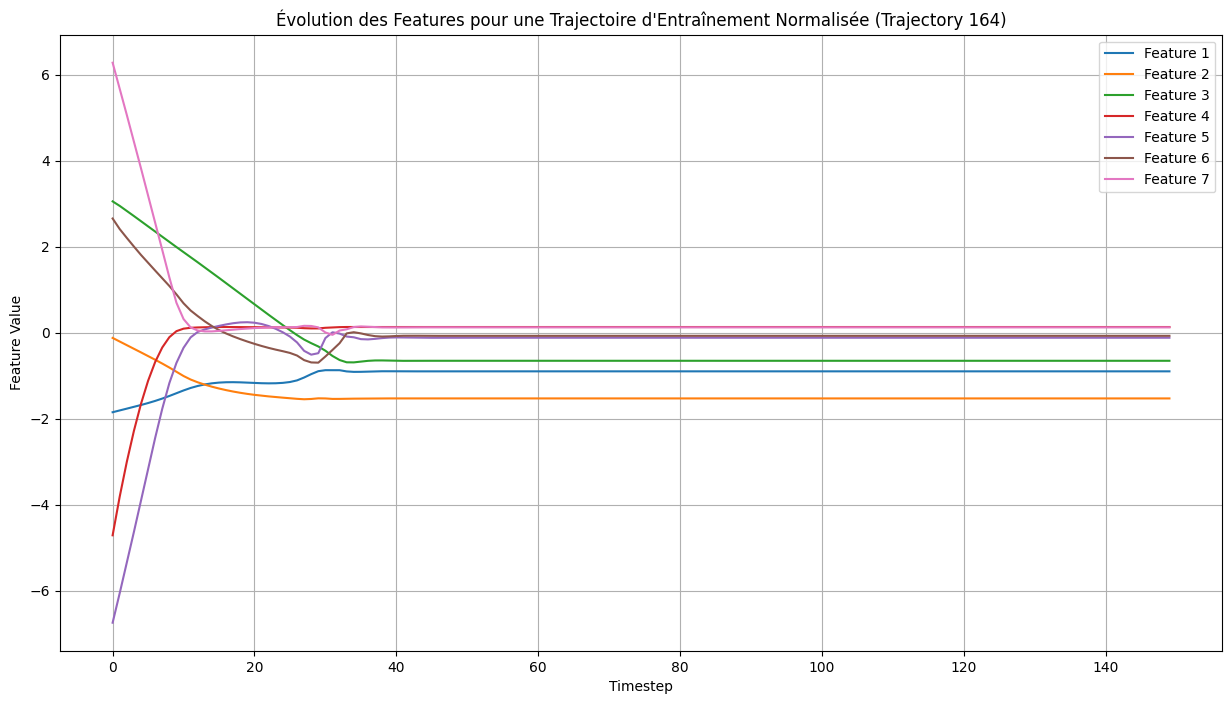
\includegraphics[width=\linewidth]{feature_effects/peg_pose_01_cell2.png}
  {\scriptsize Evolution of the 7 peg pose/orientation features.}
  \column{0.40\textwidth}
  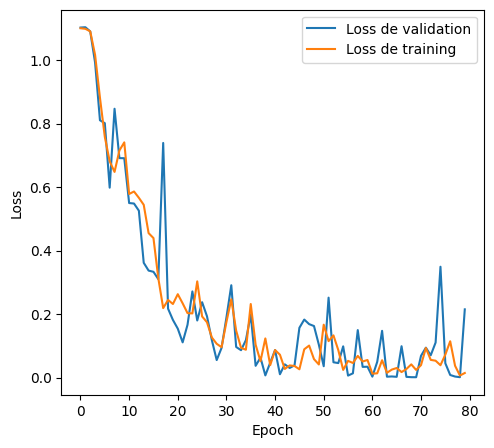
\includegraphics[width=\linewidth]{feature_effects/peg_pose_04_cell18.png}
  {\scriptsize Example loss curve (80 epochs).}
\end{columns}
\vspace{0.3em}
\footnotesize
\begin{itemize}[<+->]
  \item Test performance: 98.72\% (40 ep), 100\% (80 ep), 100\% (150 ep).
  \item Interpretation: peg pose/orientation alone already contains most class-discriminative signal.
\end{itemize}
\end{frame}

\begin{frame}{Subset B: Peg Velocities Only (7:13)}
\begin{columns}[t,onlytextwidth]
  \column{0.48\textwidth}
  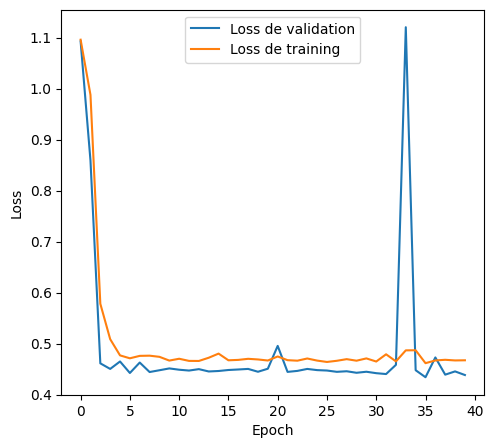
\includegraphics[width=\linewidth]{feature_effects/peg_velocity_02_cell35.png}
  {\tiny 40 epochs: moderate, unstable plateau.}
  \column{0.48\textwidth}
  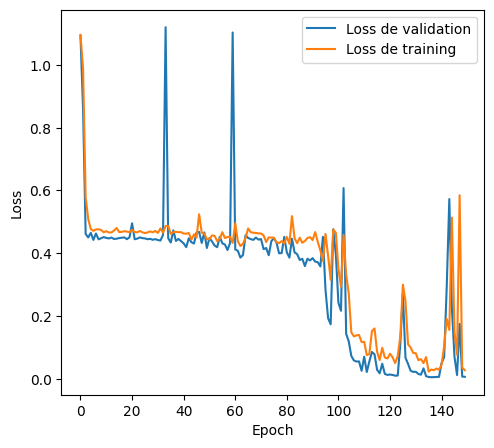
\includegraphics[width=\linewidth]{feature_effects/peg_velocity_06_cell50.png}
  {\tiny 150 epochs: late transition to low loss.}
\end{columns}
\vspace{0.2em}
\scriptsize
\begin{itemize}[<+->]
  \item Test performance: 64.10\% (40 ep), 66.67\% (80 ep), 100\% (150 ep).
  \item Two regimes: long plateau, then sharp improvement around epochs \(\sim95\text{--}110\).
  \item Velocity is informative, but optimization is harder and slower.
\end{itemize}
\end{frame}

\begin{frame}{Subset C: Hole Pose/Orientation Only (13:20)}
\begin{columns}[t,onlytextwidth]
  \column{0.56\textwidth}
  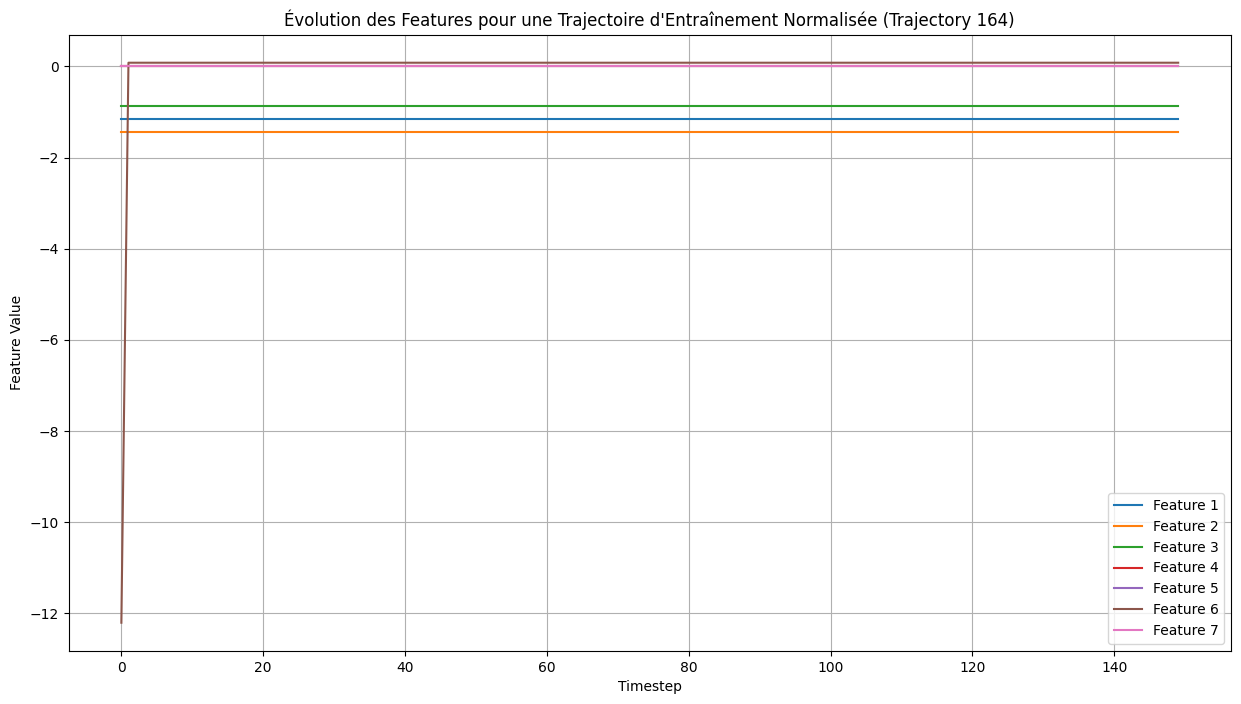
\includegraphics[width=\linewidth]{feature_effects/hole_pose_03_cell63.png}
  {\scriptsize Hole-pose features remain quasi-constant over time.}
  \column{0.40\textwidth}
  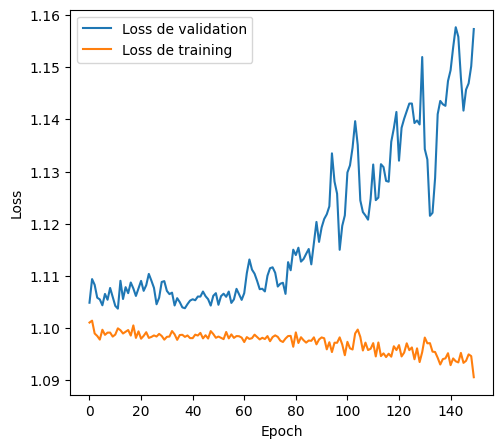
\includegraphics[width=\linewidth]{feature_effects/hole_pose_04_cell67.png}
  {\scriptsize 150 epochs: no meaningful learning.}
\end{columns}
\vspace{0.3em}
\footnotesize
\begin{itemize}[<+->]
  \item Test performance drops: 32.05\% (40 ep) \(\rightarrow\) 17.95\% (150 ep).
  \item Validation loss increases with training: more epochs worsen generalization.
  \item Interpretation: this subset is non-discriminative for this task (near-constant signal).
\end{itemize}
\end{frame}

\section{Conclusion}
\begin{frame}{Conclusion}
\small
\begin{itemize}[<+->]
  \item The final full-feature LSTM pipeline (2 layers, hidden 64, dropout, clipping) reaches top internal performance.
  \item Methodical ablation clarifies causality:
  \begin{itemize}[<+->]
    \item peg pose/orientation is highly informative,
    \item peg velocity is informative but optimization-sensitive,
    \item hole pose/orientation alone is not discriminative here.
  \end{itemize}
  \item Jury-level takeaway: good accuracy comes from both \textbf{signal selection} and \textbf{stable optimization}, not from architecture choice alone.
  \item Final validation step remains the teacher-held hidden test set.
\end{itemize}
\end{frame}

\end{document}

